% Created 2016-05-23 ma. 22:35
\documentclass[11pt]{article}
\usepackage[utf8]{inputenc}
\usepackage[T1]{fontenc}
\usepackage{fixltx2e}
\usepackage{graphicx}
\usepackage{longtable}
\usepackage{float}
\usepackage{wrapfig}
\usepackage{rotating}
\usepackage[normalem]{ulem}
\usepackage{amsmath}
\usepackage{textcomp}
\usepackage{marvosym}
\usepackage{wasysym}
\usepackage{amssymb}
\usepackage{capt-of}
\usepackage{hyperref}
\tolerance=1000
\usepackage{minted}
\usepackage{tikz}
\usepackage{parskip}
\usepackage{color}
\usepackage{listings}
\usepackage{grffile}
\definecolor{mintedbackground}{rgb}{0.95,0.95,0.95}
\usepackage[inline]{enumitem}
\usepackage{xcolor}
\hypersetup{
colorlinks,
linkcolor={red!50!black},
citecolor={blue!50!black},
urlcolor={blue!80!black}
}
\usepackage{tikz,graphics,graphicx}
\usetikzlibrary{decorations.shapes,arrows,decorations.pathreplacing,decorations.pathmorphing,backgrounds}
\usetikzlibrary{decorations.pathmorphing}
\usetikzlibrary{shapes.geometric}
\usepackage{setspace}%% The linestretch
\singlespacing
\usepackage[format=hang,indention=0cm,singlelinecheck=true,justification=raggedright,labelfont={normalsize,bf},textfont={normalsize}]{caption} %
\usepackage{vmargin}
\setpapersize{A4}
\setmarginsrb{2.5cm}{1cm}% links, oben
{2.5cm}{2cm}% rechts, unten
{12pt}{30pt}% Kopf: Höhe, Abstand
{12pt}{30pt}% Fuß: Höhe, AB
\usepackage{upquote}
%  use straight quotes when printing a command in minted
\AtBeginDocument{%
\def\PYZsq{\textquotesingle}%
}
\setlength{\parindent}{0pt}
\setlength{\parskip}{\baselineskip}
\definecolor{mintedbackground}{rgb}{0.95,0.95,0.95}
\author{Alexander Jueterbock, Martin Jakt\thanks{University of Nordland, Norway}}
\date{\textbf{PhD course: High throughput sequencing of non-model organisms}}
\title{\textbf{Genome Assembly} (June 2016)}
\hypersetup{
 pdfkeywords={},
  pdfsubject={},
  pdfcreator={Emacs 24.5.1 (Org mode 8.3beta)}}
\begin{document}

\maketitle
\tableofcontents








After removing adapters and bad-quality reads, we are ready for \emph{de
novo} assembly of the sequenced genome libraries. The number of
available genomes is increasing, also for non-model species (for
marine species, see for example \href{http://cemeb.science.gu.se/research/imago-marine-genome-projects}{The IMAGO Marine Genome
projects}). Many analyses are only possible with a reference 
genome. Thus, \emph{de novo} assembly is a first important step for many
follow-up analyses, such as SNP-discovery for population-genomics or
differential-expression analysis based on RNAseq data.

\section{MIRA - assembler}
\label{sec-1}
The choice of \emph{de novo} sequence assemblers is wide (\href{http://en.wikibooks.org/wiki/Next_Generation_Sequencing_\%28NGS\%29/De_novo_assembly#Creating_a_dataset}{overview}). Some
of the better known open-source assemblers include \href{http://bioinf.spbau.ru/spades}{SPAdes}, \href{http://www.ebi.ac.uk/~zerbino/velvet/}{Velvet},
\href{http://soap.genomics.org.cn/soapdenovo.html}{SOAPdenovo}, and \href{http://sourceforge.net/projects/mira-assembler/}{MIRA}. Have a look on \href{http://gage.cbcb.umd.edu/index.html}{GAGE}, which compares the
performance of major assembly strategies.

We use \href{http://sourceforge.net/projects/mira-assembler/}{MIRA} in this tutorial because it can handle sequencing data
from different platforms, including Illumina and Ion Torrent. Please
find its documentation \href{http://mira-assembler.sourceforge.net/docs/DefinitiveGuideToMIRA.pdf}{here}. Use the following command to get an
overview of the parameters:

\begin{minted}[fontsize=\scriptsize,bgcolor=lightgray,linenos]{sh}
mira --help
\end{minted}

Before we start, we will create a folder that contains the data we
want to assemble:

\begin{minted}[fontsize=\scriptsize,bgcolor=lightgray,linenos]{sh}
mkdir GenomeAssembly
cd GenomeAssembly
mkdir data
\end{minted}

copy your quality-trimmed fastq file into the \texttt{data} directory with:

\begin{minted}[fontsize=\scriptsize,bgcolor=lightgray,linenos]{sh}
cp SOURCEFILE TARGETDIRECTORY
\end{minted}

Here, you have to replace \texttt{SOURCEFILE} with your trimmed fasta files
and \texttt{TARGETDIRECTORY} with the path to the \texttt{data} directory that you just created.
In case of paired-end sequencing, you copy both the fasta file with
trimmed forward reads and the fasta file with trimmed reverse reads
into this folder.



The configurations for \texttt{mira} are specified in a so-called \texttt{manifest}
file. In this tutorial and will choose the most simple settings for a
\emph{de novo} genome assembly.




To create the manifest file in your \texttt{GenomeAssembly} directory, use
the command \texttt{touch}:

\begin{minted}[fontsize=\scriptsize,bgcolor=lightgray,linenos]{sh}
touch manifest.conf
\end{minted}

Now, to edit this file, we can use the command-line program
\texttt{nano}. This allows you to open and edit small text files from the command
line (no graphical user interface needed). To open the \texttt{manifest.conf}
file, just type:

\begin{minted}[fontsize=\scriptsize,bgcolor=lightgray,linenos]{sh}
nano manifest.conf
\end{minted}

Once you hit ENTER, \texttt{manifest.conf} will be opened. For now, it is
still empty. You can edit the content of the file by deleting and
adding text. At the bottom of the terminal window you see some
shortcuts for certain actions. For example \texttt{\textasciicircum{}O WriteOut} or 
\texttt{\textasciicircum{}X Exit}. The \texttt{\textasciicircum{}} indicates that you need to press CTRL+O or CTRL+X.

Depending on whether you have sequencing data from Illumina or from
Ion Torrent, your \texttt{manifest.conf} file should have different
content. Each case is described in the folllowing two sections.

\subsection{manifest file for Ion Torrent data}
\label{sec-1-1}
\begin{minted}[fontsize=\scriptsize,bgcolor=lightgray,linenos]{sh}
# Manifest file for de novo genome assembly with Ion Torrent single reads

project = IonTorrentDeNovoAssembly
job = denovo,genome,accurate

readgroup = UnpairedIonTorrentReadsFromHTSCourse2015
data = fastq::data/YOURINPUTFILE.fq
technology = iontor
\end{minted}

You can copy these lines and paste them into your file by pressing
SHIFT+CTRL+V. Change the name \texttt{YOURINPUTFILE.fq} to the name of the
fastq-file that contains your quality-trimmed reads. Then save the
file and exit with CTRL+O and CTRL+X.

That's all you need before you can start \texttt{mira} with:

\begin{minted}[fontsize=\scriptsize,bgcolor=lightgray,linenos]{sh}
nohup mira manifest.conf >log_assembly.txt &
\end{minted}

The analysis will take at least 1 hour to finish.

\subsection{manifest file for Illumina data}
\label{sec-1-2}

The illumina runs produced paired end reads. To assemble these reads
with MIRA, we have to specify two additional parameters as compared
with single end reads:
\begin{enumerate}
\item \texttt{segment\_placement} The orientation of the forward and backward
reads to each other. In our case it is \texttt{-{}-{}-> <-{}-{}-}
\item \texttt{template\_size} The total length the fragments. The total length of
the reads is 600bp. The length of the fragments depends on the
overlap between the reads. If they overlap by 200bp, then the total
length of the fragments is 400bp. We can specify a range, like \texttt{500
   700} (for 500bp-700bp). If we are unsure about this, we can
increase the range and use the \texttt{autorefine} feature of MIRA to
automatically refine this range during the assembly based on real,
observed distances of read pairs.
\end{enumerate}

Here, we specify the manifest file as:


\begin{minted}[fontsize=\scriptsize,bgcolor=lightgray,linenos]{sh}
# Manifest file for de novo genome assembly with paired end Illumina data
project = IlluminaDeNovoAssembly
job = denovo,genome,accurate
parameters = -NW:cmrnl=warn

readgroup = PairedIlluminaReadsFromHTSCourse2015
data = fastq::data/YOURINPUTFILE_1.fq fastq::data/YOURINPUTFILE_2.fq
technology = solexa
template_size = 100 1000 autorefine
segment_placement = ---> <---
\end{minted}

The Illumina reads generally have names longer than 40
characters. MIRA stops running in this case because several programs
have restrictions concerning the length of the read name. In our case
we let MIRA give us a warning about this but avoid that the program
stops completely by providing the argument \texttt{-NW:cmrnl=warn}.


You can copy these lines and paste them into your file by pressing
SHIFT+CTRL+V. Change the name \texttt{YOURINPUTFILE\_1.fq}
\texttt{YOURINPUTFILE\_2.fq} to the name of the fastq-files that contain your
quality-trimmed forward and reverse reads. Then save the file and exit
with CTRL+O and CTRL+X.

If you do not know these parameters at all, you could simply add the
parameter \texttt{autopairing} to your manifest file, like here:

\begin{minted}[fontsize=\scriptsize,bgcolor=lightgray,linenos]{sh}
# Manifest file for de novo genome assembly with paired end Illumina data - the lazy way;)

project = IlluminaLazyDeNovoAssembly
job = denovo,genome,accurate
parameters = -NW:cmrnl=warn


readgroup = PairedIlluminaReadsFromHTSCourse2015
autopairing
data = fastq::data/YOURINPUTFILE_1.fq fastq::data/YOURINPUTFILE_2.fq
technology = solexa
-NW:cmrnl=warn
\end{minted}


That's all you need before you can start \texttt{mira} with:


\begin{minted}[fontsize=\scriptsize,bgcolor=lightgray,linenos]{sh}
nohup mira manifest.conf >log_assembly.txt &
\end{minted}


The analysis will take at least 1 hour to finish.

\section{Results and assembly metrics}
\label{sec-2}

MIRA creates a directory named \texttt{PROJECTNAME\_assembly} (you defined the
PROJECTNAME in the manifest file) and several subdirectories. We are
primarily interested in the following two subdirectories:
\begin{itemize}
\item 1. \texttt{PROJECTNAME\_d\_results}: this directory contains all the output
files of the assembly in different formats. Here we are specifically
interested in the following fasta files:
\begin{itemize}
\item \texttt{PROJECTNAME\_out.padded.fasta}. This file contains the assembled contigs. Gaps are denoted by an asterisk.
\item \texttt{PROJECTNAME\_out.unpadded.fasta}. This file also contains
the assembled contigs, but with positions containing gaps removed.
\item \texttt{PROJECTNAME\_LargeContigs\_out.fasta}. This file contains the longer contigs of
your assembly, which are of particular interest. To be included in
this file, a contig generally needs to be at least 500bp long and
must have a coverage of at least 1/3 of the average coverage.
\end{itemize}
\item 2. \texttt{PROJECTNAME\_d\_info}: this directory contains files describing the properties of
the final assembly. We are particularly interested in:
\begin{itemize}
\item \texttt{PROJECTNAME\_info\_assembly.txt}. This file contains
summary statistics and information about problematic areas in the
results. Here, 'Consensus bases with \href{http://www.bioinformatics.org/sms/iupac.html}{IUPAC}' refers to positions
that are not clearly 'A', 'C', 'T', or 'G', but where two or more
bases were equally likely. For example, 'R' refers to 'A or G', and
'K' refers to 'G or T'.
\item \texttt{PROJECTNAME\_info\_contigstats.txt}. This file
contains statistics about the contigs themselves, their length,
average consensus quality, number of reads, maximum and average
coverage, average read length, number of A, C, G, T, N, X and gaps.
\end{itemize}
\end{itemize}


Search for the following information in \texttt{PROJECTNAME\_info\_assembly.txt}:
\begin{itemize}
\item Number of contigs in the assembly
\item Maximum contig coverage
\item Largest contig
\item N50 contig size
\end{itemize}

Reminder on the N50 metric (see Fig. \ref{fig:N50}):


\begin{figure}[htb]
\centering
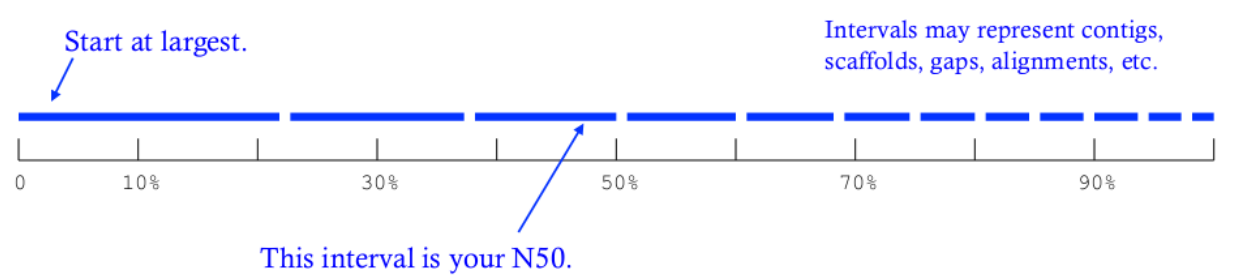
\includegraphics[width=11cm]{N50.png}
\caption{\label{fig:N50}From Kane, N.C.}
\end{figure}


N50 measures the median contig length in a set of sequences. The
larger it is, the closer your assembly gets to the real genome. N50 is
obtained by:
\begin{itemize}
\item 1. Sorting contigs in descending length order.
\item 2. Identifying the size of the contig above which the assembly contains at least 50\% of the
total length of all contigs.
\end{itemize}


We can use the program R to create histograms of the contig lengths
and coverages from the file
\texttt{PROJECTNAME\_info\_contigstats.txt}. If you are in the
directory named \texttt{PROJECTNAME\_assembly} (if you are not in
this directory, you can move to it with the \texttt{cd} command), you can
copy and paste the following commands into your terminal window to
plot histograms of the contig lengths and coverages:

Replace here PROJECTNAME with the name of your own project. For this,
you can first copy all of the following commands besides the last line
(\texttt{R CMD BATCH...}) and past it in your terminal. Then you can use
\texttt{nano Rplothistogram.r} to change the contents of this file.

\begin{minted}[fontsize=\scriptsize,bgcolor=lightgray,linenos]{sh}
rm Rplothistogram.r # Use this if the file Rplothistogram.r already exists.

cat >> Rplothistogram.r << 'EOF'
contigs <- read.table(
  file="PROJECTNAME_d_info/PROJECTNAME_info_contigstats.txt", 
  sep="\t", header=FALSE)

png(filename = "ContigLengths.png",
  width = 480, height = 480, units = "px", pointsize = 12,
  bg = "white")
hist(contigs$V2,main="Histogram of contig lengths",
  xlab="Contig length (bp)",ylab="Frequency",col="blue",breaks=100)
dev.off()

png(filename = "ContigCoverages.png",
  width = 480, height = 480, units = "px", pointsize = 12,
  bg = "white")
hist(log10(contigs$V6),main="Histogram of average log10 contig coverages",
  xlab="Average log10 contig coverage",ylab="Frequency",col="blue",breaks=100)
dev.off()

EOF

R CMD BATCH Rplothistogram.r
\end{minted}



Alternatively you can use R interactively by starting an R session
(just type \texttt{R} and return) and pasting the commands one by one into the
R session. In this case you can omit the \texttt{png(...)} and \texttt{dev.off()} commands;
these are used to create exportable images of plots (see below for more).

To open the figures, you can use the \texttt{eog} command, which is the
Eye of Gnome graphics viewer program:

\begin{minted}[fontsize=\scriptsize,bgcolor=lightgray,linenos]{sh}
eog ContigLengths.png
eog ContigCoverages.png
\end{minted}


Example histograms of contig lengths and coverages are shown in
Fig. \ref{fig:histcontlength} and \ref{fig:histcontcov}.


\begin{figure}[htb]
\centering
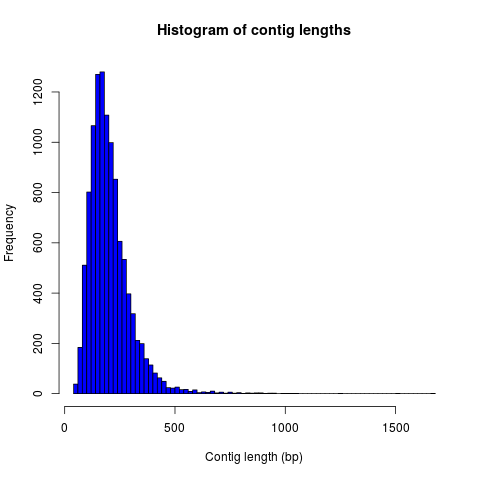
\includegraphics[width=8cm]{ContigLengths.png}
\caption{\label{fig:histcontlength}Histogram of contig lengths}
\end{figure}


\begin{figure}[htb]
\centering
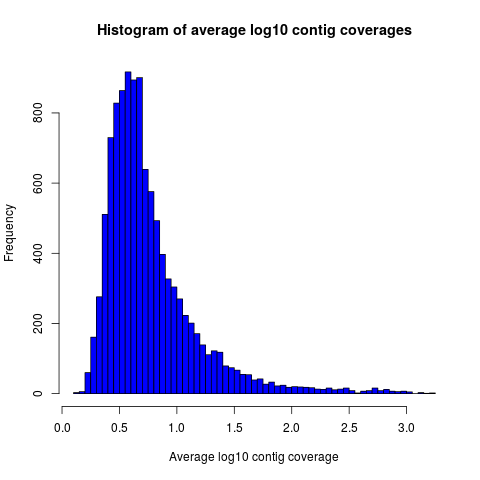
\includegraphics[width=8cm]{ContigCoverages.png}
\caption{\label{fig:histcontcov}Histogram of contig coverages}
\end{figure}

\clearpage




You can also extract the number of contigs>500bp and the sum of bases
in these contigs with R. Until now you have used R scripts with the \texttt{R
CMD BATCH} command, just like the created script \texttt{Rplothistogram.r}
above.

Instead of running \texttt{R} scripts from the shell command line, you can
also open an \texttt{R} command-line window where you can execute commands
directly. To start \texttt{R}, just type \texttt{R} in the terminal and hit
enter. All that comes after this command will be executed in the R
console. Lines preceded with a \texttt{\#}-sign will be ignored and serve only
as non-executed comments. You should be in the directory named
\texttt{PROJECTNAME\_assembly}

Again, replace here PROJECTNAME with the name of your own project.

\begin{minted}[fontsize=\scriptsize,bgcolor=lightgray,linenos]{r}
R

# open the output file from MIRA
contigs <- read.table( 
file="PROJECTNAME_d_info/PROJECTNAME_info_contigstats.txt", 
  sep="\t", header=FALSE)

# Extract only those contigs that are longer than 500bp
contigs.above500 <- contigs[contigs[,2]>500,2]

# Count the number of contigs that are longer than 500bp
length(contigs.above500)
# Output for example: 156


# Count the number of bases in these contigs
sum(contigs.above500)
# Output for example 102297

# leave R again
q()
n
\end{minted}



MIRA does not only assemble your reads but it comes with a command
line tool named \texttt{miraconvert}, which allows you to extract contigs
based on, for example, contig length and coverage (see in the \href{http://mira-assembler.sourceforge.net/docs/DefinitiveGuideToMIRA.pdf}{MIRA documentation} for further details and options).




\section{Next steps to consider}
\label{sec-3}

Hint: to identify the proportion of contigs that are protein-coding
and the proportion that may result from bacterial contamination, you
can use the Basic Local Alignment Search Tool (\href{http://blast.ncbi.nlm.nih.gov/Blast.cgi}{BLAST}) to align the
contigs to databases with known genes and proteins.

Proper annotation of a \emph{de novo} genomes is a challenging task. An
overview of the process for eukaryotes is given in
\href{http://www.marcottelab.org/users/BIO337_2014/EukGeneAnnotation.pdf}{Yandell, Mark, and Daniel Ence. "A beginner's guide to eukaryotic genome annotation." Nature Reviews Genetics 13.5 (2012): 329-342.}
If you work with prokaryotes, have a look at \href{http://stothard.afns.ualberta.ca/public_html/papers/curr_opin_microbiol_bacterial_annotation.pdf}{Stothard, Paul, and David S. Wishart. "Automated bacterial genome analysis and annotation." Current opinion in microbiology 9.5 (2006): 505-510.}

For protein annotation it helps also to sequence the
transcriptome. The assembled contigs of the transcriptome will only
consist of exons; all introns are cut out. Annotation of a \emph{de novo}
transcriptome assembly is described in \href{http://sfg.stanford.edu/BLAST.html}{The Simple Fool's Guide to
Population Genomics via RNA-Seq}. Be aware that the annotation can take several weeks to finish.

MIRA assembles the reads to so-called contigs, which are based on
overlapping sequences. Contigs can be joined with mate-pair libraries
into longer fragments (often referred to as scaffolds, which are
basically contigs that were connected by gaps, see figure below). MIRA
does not perform scaffolding. This can be done with the stand-alone
\href{http://www.baseclear.com/genomics/bioinformatics/basetools/SSPACE}{SSPACE} software.


\begin{center}
\begin{figure}[htb]
\setlength{\belowcaptionskip}{-1cm}
\scalebox{0.5}{
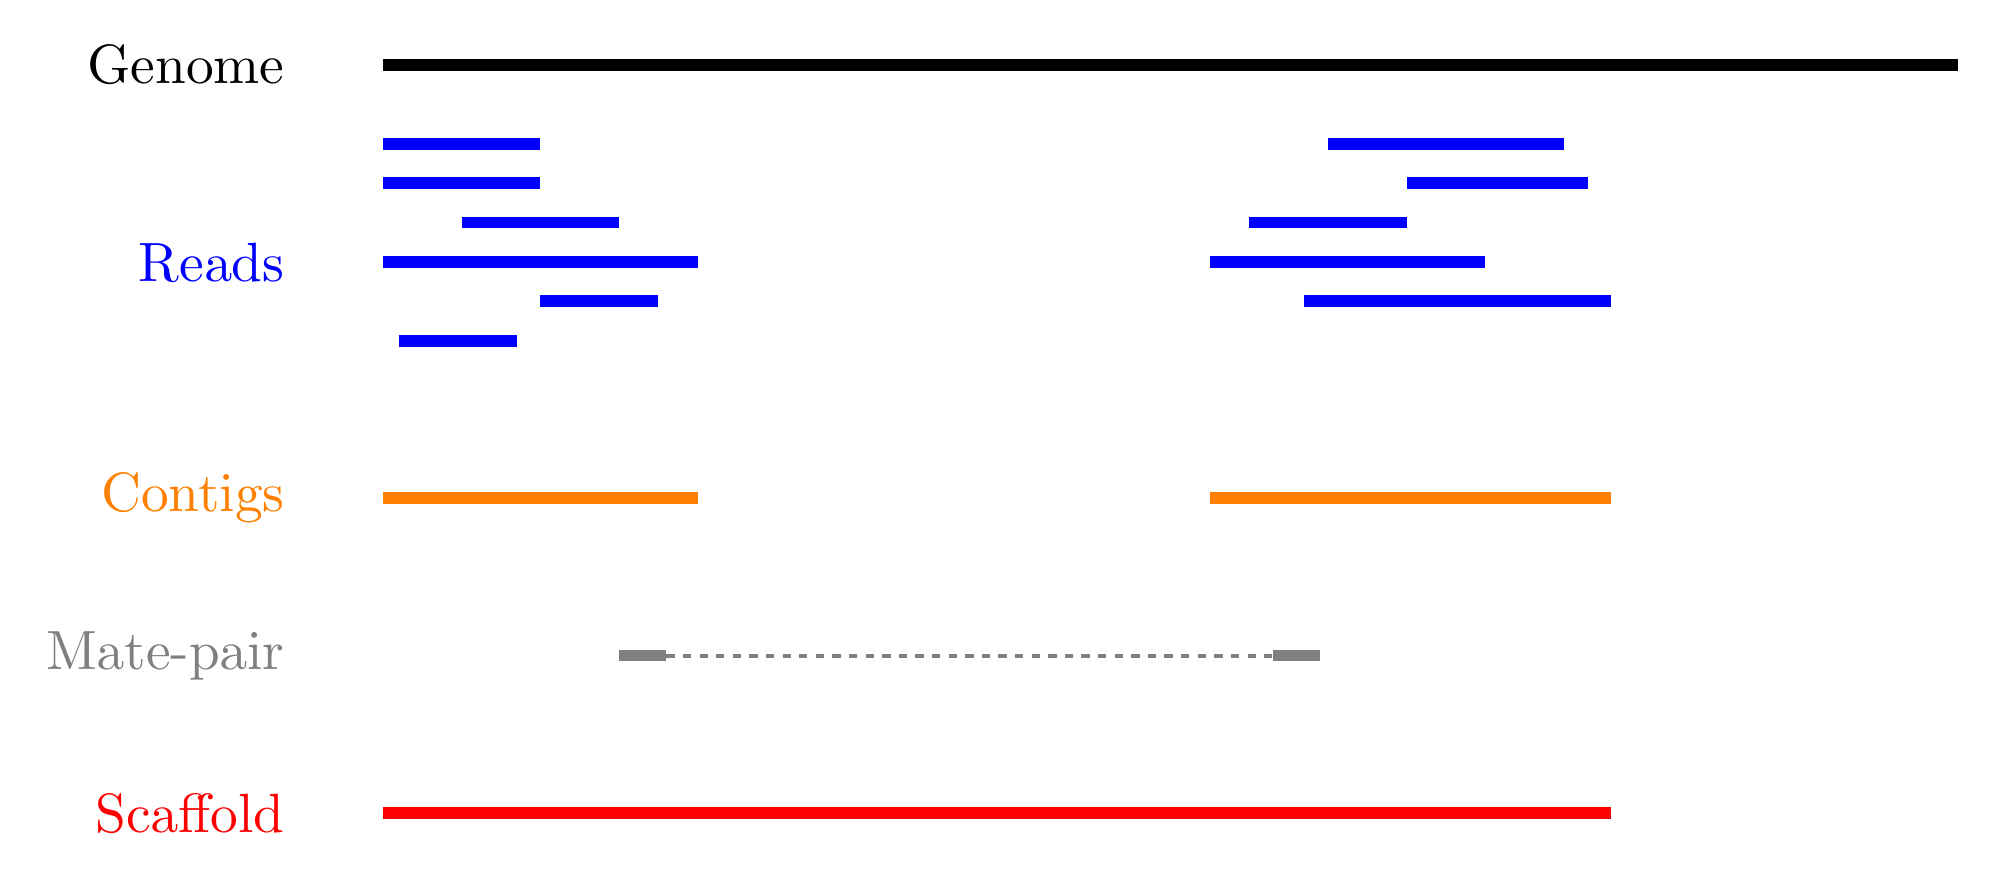
\begin{tikzpicture}

\node [anchor=east, scale=2] at (-1cm, 0.5cm) {Genome};
\node [anchor=east, scale=2,color=blue] at (-1cm, -2cm) {Reads};
\node [anchor=east, scale=2,color=orange] at (-1cm, -5cm) {Contigs};
\node [anchor=east, scale=2,color=gray] at (-1cm, -7cm) {Mate-pair};
\node [anchor=east, scale=2,color=red] at (-1cm, -9cm) {Scaffold};

\draw [line width=0.15cm, anchor=west] (0cm,0.5cm) -- (20cm,0.5cm);


\draw [line width=0.15cm, anchor=west,color=blue] (0cm,-0.5cm) -- (2cm,-0.5cm);
\draw [line width=0.15cm, anchor=west,color=blue] (0cm,-1cm) -- (2cm,-1.cm);
\draw [line width=0.15cm, anchor=west,color=blue] (1cm,-1.5cm) -- (3cm,-1.5cm);
\draw [line width=0.15cm, anchor=west,color=blue] (0cm,-2cm) -- (4cm,-2cm);
\draw [line width=0.15cm, anchor=west,color=blue] (2cm,-2.5cm) -- (3.5cm,-2.5cm);
\draw [line width=0.15cm, anchor=west,color=blue] (0.2cm,-3cm) -- (1.7cm,-3cm);

\draw [line width=0.15cm, anchor=west,color=blue] (12cm,-0.5cm) -- (15cm,-0.5cm);
\draw [line width=0.15cm, anchor=west,color=blue] (13cm,-1cm) -- (15.3cm,-1cm);
\draw [line width=0.15cm, anchor=west,color=blue] (11cm,-1.5cm) -- (13cm,-1.5cm);
\draw [line width=0.15cm, anchor=west,color=blue] (10.5cm,-2cm) -- (14cm,-2cm);
\draw [line width=0.15cm, anchor=west,color=blue] (11.7cm,-2.5cm) -- (15.6cm,-2.5cm);

\draw [line width=0.15cm, anchor=west,color=orange] (0cm,-5cm) -- (4cm,-5cm);
\draw [line width=0.15cm, anchor=west,color=orange] (10.5cm,-5cm) -- (15.6cm,-5cm);

\draw [line width=0.15cm, anchor=west,color=gray] (3cm,-7cm) -- (3.6cm,-7cm);
\draw [line width=0.05cm, dashed, anchor=west,color=gray] (3.6cm,-7cm) -- (11.3cm,-7cm);
\draw [line width=0.15cm, anchor=west,color=gray] (11.3cm,-7cm) -- (11.9cm,-7cm);

\draw [line width=0.15cm, anchor=west,color=red] (0cm,-9cm) -- (15.6cm,-9cm);

\end{tikzpicture}
} 
\end{figure}
\end{center}
Emacs 24.5.1 (Org mode 8.3beta)
\end{document}